\chapter{Theoretical background}
\label{Chapter2}

\noindent
This chapter introduces the theoretical foundation
for describing the dynamics in a system of $N$ atoms that interact with a radiation field.
First, the theory of open quantum systems is presented, which allows for the description of a general quantum mechanical system interacting with its environment.
Using this framework, the interaction between atoms and light can be analyzed.
An important phenomenon in this context is collective dissipation, particularly sub- and superradiance, which is explained in \autoref{sec:Coherent_Dissipation}.
Additionally, \autoref{sec:Green_tensor} introduces a mathematical tool for describing the electromagnetic field: the Green's tensor.
Now all tools are laid out to describe the open atomic system.
An effective equation for a single photonic excitation in a system of $N$ atoms is derived in \autoref{sec:Adapt_to_System}.
The evolution depends on the geometry of the system.
Finally, the chapter discusses the important example of an atomic lattice.
In this case, the analysis can be extended to the so-called reciprocal space, which enables tuning the transport properties of the excitation.
This is important for \autoref{Chapter4}, where an excitation will be transported on a topology of three connected chains.



%----------------------------------------------------------------------------------------
%	SECTION 2
%----------------------------------------------------------------------------------------
\section{\textbf{O}pen \textbf{Q}uantum \textbf{S}ystems} \label{sec:OQS}
Every real-world quantum system $\text{S}$ (except for the whole universe) is inevitably interacting with an environment/a bath $\text{B}$.
This interaction introduces additional degrees of freedom that influence the system's behavior, complicating its analysis.
An effective equation of motion, the so-called Lindblad master equation, is found for the (sub-)system of interest $\text{S}$.
Detailed derivations of this equation can be found in \cite{Breuer2002, Manzano_2020}.
The main ideas are outlined here.

\noindent
The combined Hamiltonian of the system is given by

\begin{equation} \label{eq:Hamiltonean_H_S_H_B_H_I}
\hat{H} = \hat{H}_{\text{S}} + \hat{H}_{\text{B}} + \hat{H}_{\text{I}},
\end{equation}

\noindent
where $\hat{H}_{\text{S}}$ ($\hat{H}_{\text{B}}$) act only on the Hilbert spaces of $\text{S}$ ($\text{B}$) respectively, and $\hat{H}_{\text{I}}$ describes their interaction.
In the Dirac picture, a state only evolves, according to the time-evolution operator $ \hat{U} $ with the non-interacting Hamiltonian
$\hat{H}_{\text{0}} = \hat{H}_{\text{S}} + \hat{H}_{\text{B}}$.

\noindent
A stochastic quantum state can be described by a density matrix $\hat{\rho}$.
In the Dirac (also called interaction-) picture,
the evolution of the total density matrix $\hat{\rho}$ is given by the Liouville-von Neumann equation \cite{Manzano_2020}

\begin{equation}\label{eq:Liouville_v_N}
\frac{d\hat{\rho}(t)}{dt} = -\frac{i}{\hbar}  \left[ \hat{H}'_I(t), \hat{\rho}(t) \right],
%\frac{d}{dt} \left( \hat{U}(t) \hat{\rho}' \hat{U}(t)^{\dagger} \right) = -\frac{i}{\hbar} \left[ \hat{H}, \hat{U}(t) \hat{\rho}' \hat{U}(t)^{\dagger} \right],
\end{equation}

\noindent
where $\hat{H}'_I(t) = \hat{U}^{\dagger} \hat{H}_I \hat{U}$
with the time-evolution operator

\begin{equation} \label{eq:Time_evolution_op}
\hat{U}(t) = \exp \left[ -\frac{i}{\hbar} \left( \hat{H}_{\text{S}} + \hat{H}_{\text{B}} \right) t \right] \text{.}
\end{equation}

\noindent
The idea is to integrate \autoref{eq:Liouville_v_N} and then apply the following approximations \cite{Breuer2002}.
First the \textbf{Born approximation} assumes that the interaction $\hat{H}_{\text{I}}$ between the bath and the system is small.
The \textbf{Markov approximation},
which assumes that bath correlations decay on a much shorter timescale than any relevant dynamics of the system,
allows one to write the total state at time $t = 0$ as a tensor product of two states.
These correspond to the fast and slow variables $\hat{\rho} = \hat{\rho}_{\text{S}} \otimes \hat{\rho}_{\text{B}}$.
The correlations of the bath can thus be traced out, and $\text{tr}_\text{B}[\hat{H}'_I(t), \hat{\rho}(0)]=0$.
Finally, using the \textbf{secular approximation} then leads to an equation in Lindblad form by averaging over very fast oscillating terms.
In the Schrödinger picture, one obtains a general master equation in Lindblad form

\begin{equation}\label{eq:ME_in_Linblad_form}
\frac{d\hat{\rho}_\text{S}}{dt} = -\frac{i}{\hbar} [\hat{H}, \hat{\rho}_\text{S}] + \sum_k \Gamma_k \left( \hat{L}_k \hat{\rho}_\text{S} \hat{L}_k^{\dagger} - \frac{1}{2} \left\{ \hat{L}_k^{\dagger} \hat{L}_k, \hat{\rho}_\text{S} \right\} \right) \text{,}
\end{equation}

\noindent
with $ \hat{L}_k $ being the so-called jump operators that
represent some non-unitary process.
%They are found as the eigenstates of the $N \times N$ interaction matrix $\Gamma$ which will be defined later.
The master equation can be rewritten in terms of an $N \times N$ interaction matrix $\Gamma$ which will be defined later.
The corresponding eigenvalues $ \Gamma_k $ reflect how frequently such a jump occurs \cite{Campaioli2024}.
From now on just $ \hat{\rho} $ will be used instead of $ \hat{\rho}_{\text{S}} \equiv  \text{tr}_\text{B}(\hat{\rho})$ to denote the density matrix of the subsystem S.

%----------------------------------------------------------------------------------------
%	SECTION 1
%----------------------------------------------------------------------------------------
\section{Collective dissipation}\label{sec:Coherent_Dissipation}
%\todo{\cite{Longo2016}} I would say, this is not needed anymore
\noindent
To understand dissipation of multiple atoms,
it is crucial to first describe the single atomic behavior.
A single atom that interacts with an electromagnetic field undergoes spontaneous emission.
This is characterized by the rate $\gamma$, with which the probability of finding the atom in an initially excited state decays.
Such an atom can be effectively described as a two-level quantum system.
This idealization is commonly realized by tuning a laser near the resonance frequency of the atomic transition, given by $ \omega_0 = c k = 2 \pi c / \lambda_0 $.
The two-dimensional Hilbert space $\mathcal{H}$ of such a Qubit is spanned by a ground state $\vert g \rangle$
and an excited state $\vert e \rangle$.
This system can be treated with the theory of open quantum systems which results in the master equation \cite{Manzano_2020}

\begin{equation}\label{eq:1atomME}
    \frac{d\hat{\rho}}{dt} = -\frac{i}{\hbar} [\hat{H}, \hat{\rho}] + \gamma \left( \hat{\sigma} \hat{\rho} \hat{\sigma}^\dagger - \frac{1}{2} \left\{ \hat{\sigma}^\dagger \hat{\sigma}, \hat{\rho} \right\} \right) ,
\end{equation}
where $ \hat{H} $ describes the unitary evolution of the atom and $  \hat{\sigma} = \vert g \rangle \langle e \vert $ is the atomic lowering operator and its hermitian conjugate $ \hat{\sigma}^\dagger $ the raising operator.

\noindent
This work extends the analysis to systems involving multiple atoms.
Dicke\footnote{Robert H. Dicke (1916--1997) was a prominent American physicist
    who made significant contributions to several fields, including quantum optics, cosmology, and gravitation.
    Dicke's work from 1954 \cite{Dicke1954} laid the groundwork for understanding collective atomic behaviors
    and has since been fundamental in many-body quantum optics.} first introduced
that if $N \geq 2$ quantum objects are confined in a volume,
collective decay processes appear.
The conditions being that the volume is comparable to the dimensionality of the system and that the emitters couple to a common electromagnetic environment.
The quantum objects interact with each other via the exchange of photons and cannot be treated as independent emitters.
Thus, also the radiation of this "super atom" becomes collective.
Coherence in the emitter system itself \cite{Benedict1996} drastically changes the known single atomic decay behavior
and is the reason for the so-called “(Dicke) sub-/ superradiance”.
The emitters synchronize by either de- or constructively interfering with each other to emit at a lower / higher rate \cite{Masson2022}.
These two cases will now be distinguished.


\noindent
Superradiance typically occurs when a collection of quantum emitters (such as molecules and atoms \cite{GROSS1982301} or quantum dots \cite{Lodahl2004}) are inverted (initially mostly excited) \cite{RubiesBigorda2022}.
Then, one observes that the decay rate of the photon on the collective system $ \Gamma_{\text{eff}} $ is enhanced relative to that of a single atom, that means $\Gamma_{\text{eff}} > \gamma$.
This phenomenon is central to modern quantum optics
and has been used to reverse engineer quantum systems for applications \cite{Longo2016},
such as building lasers that operate with very few photons \cite{Bohnet2012}.
The coupled atoms here rapidly release energy within a photon burst.
Subradiance represents a mechanism for creating states with extended lifetimes $\tau_{\text{eff}} = 1 / \Gamma_{\text{eff}} \gg 1 / \gamma$.
The decay of an excitation is suppressed.
This effect was the focus of many studies in recent years.
The hope for a good excitation storage was one motivation for this research \cite{AsenjoGarcia2017, Jen2016}.
In this case, usually a single excitation is shared between closely spaced emitters \cite{AsenjoGarcia2017}.
%However, these states are very sensitive to noise [_todo_] and thus tough to detect experimentally \cite{Bellomo2017}.
Subradiant modes also offer enhanced sensitivity to external fields, which motivates the application for metrology \cite{Facchinetti2018, Ostermann2013, Plankensteiner2015}.
Subradiance was already observed in a variety of systems.
These include molecules \cite{Takasu2012, McGuyer2015}, ions \cite{DeVoe1996} and cold atomic clouds \cite{Guerin2016, Das2020}.
%Zhen Wang et al. demonstrated, that a switching between sub- and superradiant modes is possible \cite{Wang2020}.
A protocol to transport a subradiant photon will be described in \autoref{sec:Sys_def_N_bigger_6}.

\noindent
Next, a mathematical description for the propagator of the electromagnetic field will be derived.
It allows the couplings between the atoms and the field to be modeled in \autoref{sec:Single_Excitation}.



%-----------------------------------
%	SECTION 3
%-----------------------------------
\section{Green's tensor} \label{sec:Green_tensor}
The classical electromagnetic Green's function $\mathbf{G}(\mathbf{r}, \mathbf{r}', \omega)$ solves the inhomogeneous \\Helmholtz equation \cite{Asenjo-Garcia2017}

\begin{equation} \label{eq:Green_Defining_prop}
\nabla \times \nabla \times \mathbf{G}(\mathbf{r}, \mathbf{r}', \omega) -
\frac{\omega^2}{c^2} \epsilon(\mathbf{r}, \omega) \mathbf{G}(\mathbf{r}, \mathbf{r}', \omega) = \delta(\mathbf{r} - \mathbf{r}') \mathbb{1} \text{.}
\end{equation}

\noindent
Here $\epsilon(\mathbf{r}, \omega)$ is the dielectric function and $\delta$ is the Dirac delta function.
In free space, the dielectric function $\epsilon(\mathbf{r},\omega)$ is zero, which means that the Green's tensor is analytically given.
Specifically, for discrete atomic positions, one can write the Green's tensor evaluated at the positions of two atoms $\mathbf{r}_\alpha$ and $\mathbf{r}_\beta$ as

\begin{align} \label{eq:Green_vacc}
    \mathbf{G}(\mathbf{x}_\gamma, k_0 = \omega_0 / c = 2\pi / \lambda_0) = &
    \frac{e^{ik_0 \vert\mathbf{x}_\gamma\vert}}{4\pi k_0^2 \vert\mathbf{x}_\gamma\vert^3} \bigg[
    \left(k_0^2 \vert\mathbf{x}_\gamma\vert^2 + ik_0 \vert\mathbf{x}_\gamma\vert - 1\right) \mathbb{1} \nonumber \\
    & + \left(-k_0^2 \vert\mathbf{x}_\gamma\vert^2 - 3ik_0 \vert\mathbf{x}_\gamma\vert + 3 \right)
    \frac{\mathbf{x}_\gamma \times \mathbf{x}_\gamma}{\vert\mathbf{x}_\gamma\vert^2} \bigg] \text{,}
\end{align}

\noindent
describes the effects of their interactions mediated by the electromagnetic field.
To shorten the expression,
the separation vector $\mathbf{x}_\gamma \equiv \mathbf{r}_\alpha - \mathbf{r}_\beta$ between the emitters was used.
$\mathbb{1}$ denotes the three-dimensional identity matrix.
$k_0$ is the amplitude of the wave vector of the atomic transition.


\noindent
Now all tools are laid out to describe the open dynamics of the $N$-atom system interacting with a photonic environment.



%----------------------------------------------------------------------------------------
%	SECTION 4
%----------------------------------------------------------------------------------------
\section{Atomic system}\label{sec:Adapt_to_System}
The goal of this section is to apply the previous ideas to a system $ \text{S} $ of $ N $ identical two level atoms
that are weakly coupled to a common radiation field (the bath $\text{B}$).
% commonfield means, that the atoms are close together SOURCE??!?!?
The atoms are labeled with greek subscripts $ 1 \text{, ..., } \alpha \text{, ..., } N $.
In this work, atoms are assumed to be tightly confined in free space,
and the motion of the atomic sites $ \mathbf{r}_\alpha $ is therefore neglected.
This can be achieved by using laser-generated dipole-traps \cite{GRIMM200095}.
The system considers only spontaneous emission and electric dipole interactions, with each atom possessing the same two energy levels $ \vert g \rangle $ and $ \vert e \rangle $ (see \autoref{fig:dipoles}).

\begin{figure}[ht]
    \centering
    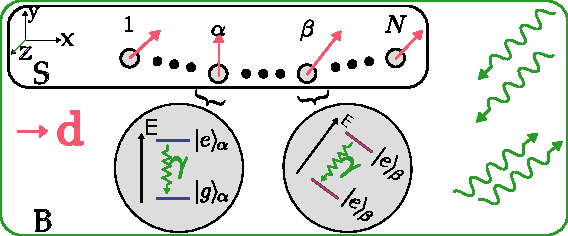
\includegraphics[width=0.6\textwidth]{N_atoms_w_dipoles}
    \caption{System S of $ N $ identical atoms, coupled to an electromagnetic bath B.
    Each carries one classical dipole-vector.
    It corresponds to the transition from the excited state $ \vert e \rangle_\alpha $ to the ground state $ \vert g \rangle_\alpha $,
    and points from the center of negative charge to the center of positive charge in the spatial distribution of the states.
    Each atom independently is subject to spontanious emission with rate $ \gamma $.}
    \label{fig:dipoles}
\end{figure}

\noindent
For the system $ \text{S} $ the quantum optical Linblad master equation
contains jump operators $\hat{L}_k$
responsible for the collective photon emission and a Hamiltonian

\begin{equation} \label{eq:Dipole_Dipole_interaction}
\hat{H}_{\text{dd}} = \hbar \sum_{\alpha, \beta} V_{\alpha\beta} \hat{\sigma}_{\alpha}^{\dagger} \hat{\sigma}_{\beta},
\end{equation}

\noindent
that represents the unitary exchange of a photon between two emitters, %(flip-flop)
%This coupling of two atoms occurs with the rate $ V_{\alpha\beta} $.
%-> not true?
with a $N \times N$ dipole-dipole interaction matrix  \(V\).
In this expression $ \hat{\sigma}_{\alpha} $ represents the lowering operators for the $\alpha$-th atom
while every other atom remains unchanged

\begin{equation}
    \hat{\sigma}_\alpha = |g_\alpha\rangle\langle e_\alpha| \equiv 1 \otimes \cdots \otimes 1 \otimes |g\rangle_\alpha \langle e|_\alpha \otimes 1 \cdots \otimes 1.
\end{equation}

\noindent
The diagonal elements of \(V\) correspond to self-interactions
like the so-called Lamb shift (caused by vacuum fluctuations of the radiation field)
which slightly alters the energy levels of the atoms.
These effects are small compared to the collective behaviors like the dipole-dipole interactions,
as this work focuses on a low-energy regime.
Therefore, they are neglected by setting \(V_{\alpha \alpha} = 0\) for all \(\alpha\) \cite{Asenjo-Garcia2017, Ma2024}.
%This interaction makes the atoms “distinguishable” from each other and reduces the high correlation of the pure symmetrical states, leading to the effect of subradiance in this system \cite{GROSS1982301}.
%I dont understand this sentences above

\noindent
The single atom lowering operators are connected to the collective jump operators via a superposition

\begin{equation}
    \hat{L}_k = \sum_{\alpha=1}^{N} c_{k, \alpha} \hat{\sigma}_{\alpha},
    \quad \text{where} \quad
    \sum_{\alpha=1}^{N} c_{k, \alpha}^* c_{\mu, \alpha} = \delta_{k\mu}
    \quad \text{and} \quad
    \sum_{k=1}^{N} \Gamma_k |c_{k,\alpha}|^2 = \Gamma_0,
\end{equation}

\noindent
where $\delta_{k\mu}$ is the Kronecker delta and $c_{k,\alpha}$ the spatial profile of the $k$-th jump operator \cite{Masson2022}.

\noindent

\noindent
As mentioned earlier,
the master equation (the extension of Eq. \eqref{eq:1atomME} to $N$ atoms)
can be rewritten with the use of a matrix $\Gamma$ as \cite{Clemens2003}

\begin{equation}\label{eq:QuantumOptical_ME}
\frac{d\hat{\rho}}{dt} = -\frac{i}{\hbar} [\hat{H}_{\text{dd}}, \hat{\rho}] + \sum_{\alpha,\beta} \Gamma_{\alpha\beta} \left( \hat{\sigma}_{\beta} \hat{\rho} \hat{\sigma}_{\alpha}^\dagger - \frac{1}{2} \left\{ \hat{\sigma}_{\alpha}^\dagger \hat{\sigma}_{\beta}, \hat{\rho} \right\} \right) ,
\end{equation}

\noindent
where $ \Gamma_{\alpha\beta} $ describe the dissipative couplings between the atoms and represent the spontaneous emission of the system.

\noindent
Each operator in the master equation acts on states in the Hilbert space of dimension $2^N$.
When calculating the evolution of a photonic excitation,
a set of equations with as many equations as the dimension of the density matrix has to be solved.
The exponential scaling with the atom number leads to difficulties
for large systems (e.g. $  N > 20 $).
Because of this, for bigger systems, techniques for dimension
reduction are necessary.
The next section brings Eq.
\eqref{eq:QuantumOptical_ME}
into a tangible form via an effective Hamiltonian in order to then apply such a reduction.


%-----------------------------------
%	SUBSECTION 1
%-----------------------------------
\subsection{Effective Hamiltonian}\label{subsec:H_eff}
Each commutator and anti-commutator can be expanded, and Eq. \eqref{eq:Dipole_Dipole_interaction} inserted to obtain
\begin{equation}
\begin{aligned}
\frac{d\hat{\rho}}{dt} &= -i \sum_{\alpha , \beta} V_{\alpha\beta} \left[-  \hat{\sigma}_{\alpha}^{\dagger} \hat{\sigma}_{\beta} \hat{\rho} +  \hat{\rho} \hat{\sigma}_{\alpha}^{\dagger} \hat{\sigma}_{\beta} \right]
 + \sum_{\alpha,\beta} \frac{\Gamma_{\alpha\beta}}{2} \left( 2 \hat{\sigma}_{\beta} \hat{\rho} \hat{\sigma}_{\alpha}^\dagger - \hat{\sigma}_{\alpha}^\dagger \hat{\sigma}_{\beta} \hat{\rho} - \hat{\rho} \hat{\sigma}_{\alpha}^\dagger \hat{\sigma}_{\beta} \right)\\
&= -i \left[ \sum_{\alpha , \beta} \left( - V_{\alpha\beta} \hat{\sigma}_{\alpha}^{\dagger} \hat{\sigma}_{\beta} - \frac{i}{2} \Gamma_{\alpha\beta} \hat{\sigma}_{\alpha}^\dagger \hat{\sigma}_{\beta} \right) \hat{\rho} \right. \\
&\quad \quad \quad + \left. \hat{\rho} \sum_{\alpha , \beta} \left( V_{\alpha\beta}  \hat{\sigma}_{\alpha}^{\dagger} \hat{\sigma}_{\beta} - \frac{i}{2} \Gamma_{\alpha\beta} \hat{\sigma}_{\alpha}^\dagger \hat{\sigma}_{\beta} \right) \right] \\
&\hspace{0.48cm}   + \sum_{\alpha,\beta} \Gamma_{\alpha\beta} \hat{\sigma}_{\beta} \hat{\rho} \hat{\sigma}_{\alpha}^\dagger .
\end{aligned}
\end{equation}

\noindent
A non-Hermitian effective Hamiltonian $ \hat{\mathcal{H}}_{\text{eff}} $ can be introduced as
\begin{equation} \label{eq:H_eff}
    \hat{\mathcal{H}}_{\text{eff}} = \sum_{\alpha, \beta} \left(- V_{\alpha\beta} - \frac{i}{2} \Gamma_{\alpha\beta} \right)\hat{\sigma}_{\alpha}^{\dagger} \hat{\sigma}_{\beta}.
\end{equation}

\noindent
Now the master equation describing the atomic system simplifies to
\begin{equation}
    \frac{d\hat{\rho}}{dt} = - i \left( \hat{\mathcal{H}}_{\text{eff}} \hat{\rho} - \hat{\rho} \hat{\mathcal{H}}_{\text{eff}}^\dagger \right) + \mathcal{D}(\hat{\rho}),
\end{equation}

\noindent
with
\begin{equation}
\mathcal{D}(\hat{\rho}) = \sum_{\alpha,\beta} \Gamma_{\alpha\beta} \hat{\sigma}_{\beta} \hat{\rho} \hat{\sigma}_{\alpha}^\dagger,
\end{equation}
describing the emission of a photon.
In the following section, a restricted subspace will be found,
where the computations for calculating an evolution are significantly reduced to order $ \mathcal{O}(N) $.



%----------------------------------------------------------------------------------------
%	SUBSECTION 2
%----------------------------------------------------------------------------------------
\subsection{Dynamics in the single excitation subspace} \label{sec:Single_Excitation}
%\cite{BRANDES2005315}:Single modes
The system is initially restricted to a superposition of single excitations
$\vert e_{\alpha} \rangle \equiv \vert g\rangle_1 \otimes \cdots \otimes \vert e\rangle_\alpha \otimes \cdots \otimes \vert g\rangle_N$, for all $\alpha = 1, \ldots, N$.
This means that exactly one, unknown atom is excited.
As mentioned above, the effective Hamiltonian $\hat{\mathcal{H}}_{\text{eff}}$ is responsible for the evolution of the initial state.
Due to dissipation into the environment, the number of excitations can only decrease to zero.
Consequently, the dynamics can be described within a truncated Hilbert space spanned by the many-body ground state
$\vert G\rangle \equiv \vert g\rangle_1 \otimes \vert g\rangle_2 \otimes \cdots \otimes \vert g\rangle_N$
and the single-excitation states $\vert e_{\alpha} \rangle$ \cite{Bienaime2012}.
The dynamics in the single-excitation subspace decouple from the rest \cite{Needham2019}.
This can be seen by inserting the ansatz for the density matrix

\begin{equation}
    \hat{\rho} = \begin{pmatrix}
        \rho_{\text{GG}} & \bm{\rho}_{\text{Ge}} \\
        \bm{\rho}_{\text{eG}} & \rho_{\text{ee}}
        \end{pmatrix} \text{,}
\end{equation}

\noindent
where $\rho_{\text{GG}} = \langle G \vert \hat{\rho} \vert G \rangle$,
$\bm{\rho}_{\text{Ge}} = \langle G \vert \hat{\rho} \vert \bm{e} \rangle$,
$\bm{\rho}_{\text{eG}} = \langle \bm{e} \vert \hat{\rho} \vert G \rangle$, and
$\rho_{\text{ee}} = \langle \bm{e} \vert \hat{\rho} \vert \bm{e} \rangle$,
with $\vert \bm{e} \rangle$ being a column vector
containing all single-excitation states $\vert e_{\alpha} \rangle$.
Inserting this into Eq.~\eqref{eq:ME_in_Linblad_form}, the matrix equation

\begin{equation}
    \frac{d}{dt} \rho_{\text{ee}} = -i \left[ H_{\text{eff}} \rho_{\text{ee}} - \rho_{\text{ee}} H_{\text{eff}}^\dagger \right]
\end{equation}

\noindent
is obtained with a new effective Hamiltonian

\begin{equation} \label{eq:reduces_H_eff}
    H_{\text{eff}} = V - \frac{i}{2} \Gamma,
\end{equation}

\noindent
where $ V $ and $ \Gamma $ are the matrices
with entries $V_{\alpha \beta}$ and $\Gamma_{\alpha \beta}$ respectively.
They are of size $N \times N $, which significantly reduces the computational power needed to calculate the time evolution of a state.

\noindent
In this subspace, the atoms can equivalently be treated like classical dipoles \cite{AsenjoGarcia2017},
which justifies the usage of $\mathbf{d}$ in \autoref{fig:dipoles}.
The dipole vector of an atom is defined by the matrix elements of the quantum mechanical dipole operator $\hat{\mathbf{d}} = q \mathbf{\hat{r}} $. %\cite{Asenjo-Garcia2017}.
The dipole vector corresponding to the transition of the $\alpha$-th atom is $\mathbf{d}_\alpha = _{\alpha}\langle g \vert \hat{\mathbf{d}}_\alpha \vert  e \rangle_{\alpha}$.


\noindent
The coefficients $V_{\alpha \beta}$ and $\Gamma_{\alpha \beta}$ can be calculated by the real and imaginary part of
$\mathbf{G}$ (which is analytically given by Eq. \eqref{eq:Green_vacc}) \cite{Asenjo-Garcia2017}

\begin{equation}\label{eq:V_matrix}
V_{\alpha \beta} = \frac{\omega_\alpha^2}{\hbar \epsilon_0 c^2}\mathbf{d}_\alpha^T \mathrm{Re}[\mathbf{G}(\mathbf{r}_\alpha, \mathbf{r}_\beta, \omega_\alpha)] \mathbf{d}_\beta
\end{equation}

\noindent
and

\begin{equation}\label{eq:Gamma_matrix}
\Gamma_{\alpha \beta} = \frac{2 \omega_\alpha^2}{\hbar \epsilon_0 c^2}\mathbf{d}_\alpha^T \mathrm{Im}[\mathbf{G}(\mathbf{r}_\alpha, \mathbf{r}_\beta, \omega_\alpha)] \mathbf{d}_\beta.
\end{equation}

\noindent
The diagonal elements of \(\Gamma\) correspond to the single-atom decay rate and can now be calculated  \(\Gamma_{\alpha \alpha} = \frac{2 \omega_\alpha^2}{\hbar \epsilon_0 c^2} \vert \mathbf{d}_{\alpha} \vert^2 \equiv \gamma\).
When the distance between atoms is comparable to the transition wavelength,
\(d \approx \lambda_0\) collective sub- and superradiance arises
(see \autoref{sec:Coherent_Dissipation}).
The off-diagonal elements satisfy \(0 \leq \Gamma_{\alpha \beta} \leq \gamma\), approaching \(\gamma\) or zero when the interatomic distance is small or large compared to the wavelength, respectively.
%In total, this matrix has positive eigenvalues.

\noindent
An effective equation of motion in the single excitation subspace was found.
With the explicit formulas for $ V $ and $ \Gamma $, that depend on the atomic transition, which is fixed, and the topology
(how the atoms are arranged and how the dipoles are orientated),
the evolution of an initial excitation on the system can be calculated.
The next section presents a measure for how good the atoms retain the excitation that is also a great tool to visualize the evolution.



%----------------------------------------------------------------------------------------
%	SUBSECTION 3
%----------------------------------------------------------------------------------------
\subsection{Survival probability}

\noindent
For the system of \( N \) atoms and for simplicity, the initial state is restricted to be a pure state, where \( \rho_{ee}(0) = \vert \psi(0) \rangle \langle \psi(0) \vert \).
Such an initial state evolves under the non-Hermitian Hamiltonian \( H_{\text{eff}} \) and stays pure.
% why can we use normal QM evolution here?? \todo
Because the Hamiltonian is time-independent, the state $\vert  \psi(t) \rangle$ can be expressed as

\begin{align} \label{eq:Phase_Decay}
\vert  \psi(t) \rangle = \exp{\left(-\frac{i}{\hbar} H_{\text{eff}} t\right)} \vert  \psi(0) \rangle =
\underbrace{\exp(-i V t)}_{\text{Phase}} \,
\underbrace{\exp(-\frac{\Gamma}{2} t)}_{\text{Decay}} \,
\vert  \psi(0) \rangle \text{.}
\end{align}

\noindent
Here the Baker–Campbell–Hausdorff formula was used to separate the operators.
The survival probability, describing the probability for not emitting a photon into the radiation field,
is given by the norm of the state described by Eq. \eqref{eq:Phase_Decay} and can be written as

\begin{equation}
    P_{\text{sur}}(t) = \vert \vert  \psi(t) \rangle \vert^2 = \sum_{\alpha=1}^{N} \vert c_{\alpha}(t) \vert^2 \text{.}
\end{equation}

\noindent
where \( \vert c_{\alpha}(t) \vert^2 \) represents the probability amplitude of the \(\alpha\)-th atom being excited at time \( t \).

\noindent
On the one hand, the matrix $ V $ contributes a phase in the evolution.
On the other hand, the equation for the density matrix is trace-preserving ($\text{Tr}[\rho] = 1$) and
$ \Gamma $ can again be connected to the dissipative dynamics, reducing the survival probability over time.
The population of the ground state $ \rho_{GG} $ increases over time.

\noindent
Thus, the survival probability quantifies how the system retains its excitation as it evolves.
It is also a great tool to visualize the evolution of a photonic excitation on the atomic system and will be used in \autoref{Chapter4}.




%----------------------------------------------------------------------------------------
%	SECTION 3
%----------------------------------------------------------------------------------------
\section{Reciprocal space} \label{sec:K-space}
The reciprocal space emerges as an important tool in the analysis of periodic systems.
Here the phase velocity can be designed for an effective excitation transport, also to be used in \autoref{Chapter4}.


\noindent
The simplest lattice is an infinitely long one-dimensional chain with sites $ \mathbf{r}_\alpha$,
and exhibits translational symmetry by any lattice vector $\mathbf{R}$.
This work focuses on the transport of an excitation on a chain of atoms.
The chain can be seen as the system S of \autoref{sec:Adapt_to_System}.
When all dipoles are aligned, the components of the Green's tensor (Eq. \eqref{eq:Green_vacc}) are translationally invariant.
Then, Blochs theorem \cite{Bloch1929} allows the diagonalization of $ \mathbf{G} $ via a Fourier transformation.
This way the eigenfunctions of $ \mathbf{G} $ can be expressed as plane waves

\begin{equation}
\vert k_i \rangle = \frac{1}{\sqrt{N}} \sum_{\alpha =1 }^{N} \langle e_\alpha \vert k_i \rangle  \vert e_\alpha \rangle
= \frac{1}{\sqrt{N}} \sum_{\alpha =1 }^{N} e^{i k_i |\mathbf{r}_{\alpha}|} \vert e_\alpha \rangle \text{.}
\end{equation}

\noindent
The Fourier transformation can be written in matrix form as

\begin{equation} \label{eq:FT}
T \equiv \left[\vert k_1 \rangle \dots \vert k_i \rangle \dots \vert k_N \rangle \right] \text{,}
\end{equation}

\noindent
and can be used to perform a change of basis between real- and reciprocal/($k$)-space.
Here $\vert k_i \rangle$ denotes the i-th eigenstate in $k$-space.
The Green's tensor is diagonal in this basis with eigenvalue $ G_{k_i} $.
One can directly connect a pseudo momentum $ k $ in the first Brillouin zone $ k \in [-\pi/d,\pi/d] \subset \mathbb{R} $ with each eigenvalue.
This reducibility comes from the fact that each state $ \vert k \rangle $ is unique up to a constant reciprocal lattice vector $\vert\mathbf{K}\vert = 2 \pi / \text{d}$.
Here $d$ is the distance of two neighboring atoms.
The real and imaginary part of the eigenvalues is directly proportional to the eigenvalues $ V_k $ and $ \Gamma_k $ respectively
(see Eqs.~\eqref{eq:V_matrix} and \eqref{eq:Gamma_matrix}).
Thus, the effective Hamiltonian Eq. \eqref{eq:reduces_H_eff}
is diagonal in $k$-space.
This relationship reveals regions of superradiance and subradiance.
Recall that superradiant modes correspond to \(\Gamma_k > \gamma\), while subradiant modes correspond to \(\Gamma_k < \gamma\).
Notably, subradiance in free space occurs for $d \leq \lambda_0/2$, at the boundaries of the Brillouin zone, away from its center.
Asenjo-Garcia et al. \cite{AsenjoGarcia2017} showed,
that the most subradiant mode decreases with the systems size $ \Gamma_{k, \text{min}} \propto N^{-3} $,
motivating the usage of a higher atomic number in \autoref{Chapter4}.
But it should be noted
that these modes are challenging
to create experimentally due to their location in \(k\)-space as well as their complicated phase pattern \cite{Cech2023}.



%----------------------------------------------------------------------------------------
%	SUBSECTION 4
%----------------------------------------------------------------------------------------
\subsection{Group velocity} \label{subsec:Phase_vel_Control}

\noindent
With Eq. \eqref{eq:Phase_Decay}, one can argue that only the V matrix defines the spectrum of the effective Hamiltonian.
By diagonalizing \(V\), one can extract the eigenenergies \(V_k\).
The phase \( \varphi \) of the evolved state in Eq. \eqref{eq:Phase_Decay} is given by

\begin{equation}
\varphi(t) \equiv V_k t + \varphi_0
\end{equation}

\noindent
where $\varphi_0$ denotes the phase of the initial state $\vert  \psi(0) \rangle$.
The gradient of the spectrum, \(V_k\), determines the dispersion relation,
which ultimately depends on atomic positions and dipole orientations.
Without loss of generality, a wave-packet $ \vert  \psi(0) \rangle $ can be localized in $k$-space.
For instance, a Gaussian wave packet in $k$-space also remains Gaussian in real space after a Fourier transform.
By controlling the shape of the wave packet in \(k\)-space, one can manipulate the behavior of excitation on the atoms.
For a sufficiently large interval with an approximately linear spectrum,
the definition of a group velocity $ v_\text{g} $ of the wave packet is possible.
This group velocity is thus proportional to the eigenenergies

\begin{equation}
    v_\text{g} \propto \nabla \varphi \equiv \nabla V_k \cdot t.
\end{equation}

\noindent
This approach also holds as a good approximation for large but finite systems,
which can be seen in \autoref{sec:Diagonalization} of the Appendix.

\noindent
One application of this is to trap photons on specific lattice sites through a flat dispersion \cite{Cech2023}.
Another application involves initializing the wave packet in a region of \(k\)-space with an approximately linear dispersion relation.
In this scenario, the wave packet propagates with a nearly constant group velocity, avoiding dispersion during its evolution \cite{Needham2019}.
By tuning the atomic chain's structure and selecting appropriate initial conditions for the wave packet, one can effectively control the phase velocity and, consequently, the dynamics of the system.